%! Suppress = MissingImport
\section{Acceptance Test Management}\label{sec:acceptance-test-management}

This section will cover the acceptance test management, mainly regarding the
scenarios, on how to write, sort and execute them.

\subsection{Cucumber scenario format}\label{subsec:cucumber-scenario-management}
% TODO some advice on cucumber scenario format

\subsubsection{Core scenario}
% TODO homemade
% TODO interact with the database, web services etc.
% TODO describe busniess rule

\subsubsection{UI scenario}
% TODO we can use NoraUI

\subsubsection{API scenario}
% TODO we can improve NoraUI for the API testing

\subsection{Scenario Tags}\label{subsec:scenario-tags}
Cucumber tag is a very helpful feature that allow us to classify our
scenarios into various categories.
This non-exhaustive section is going to present several relevant categories.

\subsubsection{Component Under Test}
We already shown an example of this tag, with the UI, API and Core scenarios.
They can be tagged using \textit{@UI}, \textit{@API} or \textit{@Core} to
indicate that they only test a specific type of component.
Hence it would be possible to easily execute the test only for the UI, which
would avoid to execute everything at the same time.

\subsubsection{Business Domain}
A tag can be added to each scenario to indicate which business domain they
belong to.
First, just like the previous tag, it allows us to execute the test of
specific business domain.
But mostly, it will serve as a hint for the documentation.

Scenarios are the living the documentation of the application.
However, when there are a lot of scenarios, it can be hard to navigate
between them and immediately understand which business domain is involved.
Hence, adding more tags like \textit{@Mailing} or \textit{@Authentication}
can be helpful.

\subsubsection{Execution Speed}
Some scenarios can be very long, when for example they involve asynchronous
computation or generate a lot of data.
These tests will inevitably slow down the entire test process and delay the
test report of the faster ones.
It's therefore interesting to add a hint about the execution speed or
resource usage like \textit{@Slow} or \textit{@Heavy}.
Their execution can be delayed so they don't block fast tests to be executed.

\subsubsection{Manual Test}
As we said earlier in the previous section of this chapter, not all the tests
can be automated, even if they can be written as a scenario.
However it's not necessarily useless to write them as a scenario, because
automation is not the only advantage of this format.
It will still contribute to the living documentation and describe the step to
do the test, using the domain vocabulary and a standard format.

Hence, manual test written as a scenario can be tagged with a
\textit{@Manual}, so we can exclude them from the automation process but
still include them as a normal scenario in the application.

\subsubsection{Current release}
Lastly, we can tag the scenario of the features that will be released in the
current version.
It will serve as an overview of what will be added and allows us to
only execute the tests of the current version, which would reduce the
execution time and feedback duration on the hot features.

\subsection{Scenario lifecycle}\label{subsec:scenario-lifecycle}
This section is going to describe the lifecycle of a scenario in our new
workflow.
We are going to take advantage of the cucumber tags to follow the state of
each scenario.

\begin{figure}
    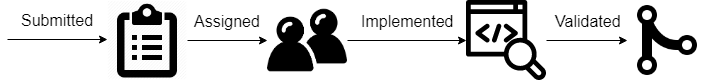
\includegraphics[width=\textwidth]{../../resources/images/solution/scenario_lifecycle.png}
    \centering
    % TODO fix position
\end{figure}

\subsubsection{Submission}
When a new scenario is written by an analyst, it is submitted in the backlog
of the dev team.
Each new scenario will be tagged with \textit{TODO} in order to easily identify
them.

\textit{@TODO} scenarios are directly added to the main branch but their
execution will be skipped in the CI jobs.
They're skipped because the tests of the main branch are always supposed to
pass.
Hence failing the job because a feature is not yet implemented would force the
team to always look at the test report and sort between not implemented
features and actual bug or regression.

\subsubsection{Assigned}
When the scenarios are assigned to a pair, a new branch is created and the
scenarios are tagged as \textit{@WIP}.
\textit{@WIP} tests are not ignored in the CI jobs, because the objective is
to turn the failing scenario to a passing one.
Therefore ignoring them would be in contradiction with our TDD approach.

When a \textit{@WIP }scenario passes, the tag should be removed.
This does not mean that the code won't be modified nor refactored, it
just indicates that the feature is correctly implemented.
The scenario now turns into a non regression test.

\subsubsection{Pending Review}
When all there is no more \textit{@WIP} tag and the code has been refactored,
the Merge Request is now ready to be reviewed.
The review is mandatory when there was only a single developer assigned to
the feature.
If it was a pair, at least two people have already seen the code, so it's
acceptable to skip the review and integrate if all the validation are
passing, like post-merge build or Sonar analysis.

\subsection{Test execution}\label{subsec:test-execution}
When there are a lot of test, especially UI tests, test execution can quickly
become very long.
Slow tests mean on one hand longer feedback but also more costly as the CI
platform will be heavily solicited and the team is likely to waste time waiting
for the build to finish.
This is why we are going to propose a new test execution strategy.

\subsubsection{Trading time}
Feedback has been a very important point throughout this solution
and most of the time, we tried to reduce at most the duration.
In this section, we're going to present why it can be interesting to
trade some feedback to save other type of resources.

We mentioned in the introduction the slow tests and their negative impact on
the CI platform and team productivity.
The thing is, running all the tests of the application for every modification
is a great for feedback, since we ensure that nothing has been broken by the
last commit.
However, this implies to execute long test suites of test, even about
completely independent modules.

A solution to reduce the execution duration could be to omit certain tests,
whether because they're slow, costly or completely unrelated.
Of course there is always a small change of regression, but sometimes it's
too small and executing on every commit is not worth.

This will also free some CI resources, which will speed up the other build
executions.
Here, we are trading feedback duration on a subset of our tests, against CI
resources and feedback duration on the hot tests, for example the tests of the
current feature and its dependent modules.

\subsubsection{On commit}
When a commit is pushed to the CI platform, a build should automatically be
triggered.
When the developer pushes a commit, he mainly wants to if its work is
correctly working on the CI platform but he also wants to know if there is no
new regression.

Here, we decided to omit the slow and unrelated tests to the build, in order
to speed up the feedback on the interesting features.
Hence, the unit and integration tests and only the WIP, core and current
release scenarios will be executed.
This ensure that the core of the application is still intact and the current
WIP features are still working correctly.

\subsubsection{Several times per day}
The tests run on every commit are only a subset of the entire application.
But there is still residual tests, like the slow and unrelated ones.
Even though some of these tests are less likely to fail, we still need to run
them.
Hence we'll do it but at a lower frequency, like every 1 or 2 hours.

These is still quick enough to catch a regression in the same day it has been
added, without extensively consuming the CI resources.

\subsubsection{Night build}
Finally, there are some tests that are very hard to run continuously.
Tests that require a fresh environment to run, or that are very long like
load would use to much resources to run during the day.
Therefore these tests can be run at night, where there is 10 hours of CI
platform fully available.
Cucumber tags can be used for this kind of tests, using a \textit{@Night} tag
to exclude them during the day.
